\documentclass[11pt]{article}
\usepackage{fullpage,fourier,amsmath,amssymb}
\usepackage{listings,color,url,hyperref}
\usepackage{epigraph}
\usepackage{graphicx}
\usepackage[x11names]{xcolor}

\title{Assignment 0 \\ \texttt{git}'n Started}
\author{Prof. Darrell Long \\ CSE 13S -- Winter 2020}
\date{Due: January  12$^\text{th}$ at 11:59\,pm}

\usepackage{fancyhdr}
\pagestyle{fancy}
\fancyhf{}

\fancypagestyle{plain}{%
  \fancyhf{}
  \renewcommand{\headrulewidth}{0pt}
  \renewcommand{\footrulewidth}{0pt}
  \lfoot{\textcopyright{} 2021 Darrell Long}
  \rfoot{\thepage}
}

\pagestyle{plain}

\definecolor{codegreen}{rgb}{0,0.5,0}
\definecolor{codegray}{rgb}{0.5,0.5,0.5}
\definecolor{codepurple}{rgb}{0.58,0,0.82}

\lstloadlanguages{C,make,python,fortran}

\lstdefinestyle{c99}{
    morekeywords={bool, uint8_t, uint16_t, uint32_t, uint64_t, int8_t, int16_t, int32_t, int64_t},
    commentstyle=\color{codegreen},
    keywordstyle=\color{magenta},
    numberstyle=\tiny\color{codegray},
    identifierstyle=\color{blue},
    stringstyle=\color{codepurple},
    basicstyle=\ttfamily,
    breakatwhitespace=false,
    breaklines=true,
    captionpos=b,
    keepspaces=true,
    numbers=left,
    numbersep=5pt,
    showspaces=false,
    showstringspaces=false,
    showtabs=false,
    tabsize=4
}

\lstset{language=C, style=c99}

\newcommand\asgn[0]{asgn0}

\begin{document}\maketitle
%%%%%%%%%%%%%%%%%%%%%%%%%%%%%%%%%%%%%%%%%%%%%%%%%%%%%%%%

\section{Introduction}
\epigraphwidth=0.75\textwidth
\epigraph{\emph{It's nice if people can finally loosen up a little bit
and just go out and laugh at silliness. I mean, people take themselves
way too seriously sometimes.}  \texttt{git}\emph{'er done!}}{---Larry the
Cable Guy}

\noindent The aim of this first assignment will be for you to set up your
\texttt{git} repositories and gain an understanding of how \texttt{git}
works. We will review several \texttt{git} commands that you will
help you in the long run. This document will be helpful for
troubleshooting \texttt{git} issues in the future and also includes
the submission policy. You will find this quite helpful in the future if you ever
have any issues with \texttt{git} or submitting.
\emph{Ideally,} this assignment
is to be completed during your discussion section.

%%%%%%%%%%%%%%%%%%%%%%%%%%%%%%%%%%%%%%%%%%%%%%%%%%%%%%%%

\section{Your Task}
\epigraph{\emph{The story of life is quicker than the wink of an eye, the
story of love is hello and goodbye\ldots until we meet again.}}{---Jimi Hendrix}

\noindent We will be creating a simple \textbf{C} program and
compiling it.  The program will simply
print \texttt{``Hello World!''}. This tutorial can also
be found in Chapter 1 \S 1.1 in your textbook, \textit{The C
Programming Language} by Kernighan \& Ritchie. At this point, you
will want to be in your \texttt{\asgn} directory as this will
be your \emph{current working directory}.

\begin{enumerate}
\item Connect to \texttt{unix.ucsc.edu} using an \texttt{ssh} client.
\item Create the program source \texttt{hello.c} with your
text editor of choice. Make sure you do this with a text
editor like \texttt{vi} or \texttt{emacs}. Notepad is \emph{not} a text editor.
For example, you would type the following into your terminal:
\begin{lstlisting}
vi hello.c
\end{lstlisting}

	\item Include the headers for the \texttt{stdio.h} library. This is needed to use \texttt{printf}.
\begin{lstlisting}
#include <stdio.h>
\end{lstlisting}

	\item Set up your \texttt{main} function.
\begin{lstlisting}
int main(void) {
  return 0;
}
\end{lstlisting}

	\item Inside the \texttt{main} function (in between the curly braces) will
        be where you will put \texttt{printf}. It is \emph{crucial} that your output matches the one given here. You will be docked points otherwise.

\begin{lstlisting}
printf("Hello World!\n");
\end{lstlisting}

	\item To compile and run this program, exit your text editor to return to the command line. For example, if you are using \texttt{vi}, you would hit the \texttt{esc} key, type ``\texttt{:wq}'' and press the Enter key. This saves your work and exits the text editor.

	\item You should be back on the command line. To compile your program, type the following line into the command line:
\begin{lstlisting}
clang -Wall -Wpedantic -Wextra -Werror hello.c -o hello\end{lstlisting}

This is also known as the ``take no prisoners'' compiler flags.
Simply put, they catch pretty much everything that a compiler can catch
(there are a few more esoteric warnings that can be
enabled). For example, the
``\texttt{-Werror}'' flag turns all warnings into errors. The ``\texttt{-Wextra}''
option warns about expressions that have no side effects and whose
value is discarded.

	\item If you've done everything correctly up to this point, the compilation
        process should run silently and return no errors. However, if you do run
        into any errors, Google, Piazza and discussion sections will be your best
        friends.

The most likely problem is that you did not use a \emph{text editor} on
\texttt{unix.ucsc.edu}---contrary to our explicit advice.

	\item After successfully compiling your program, there is now an
executable file called ``\texttt{hello}''. To run your program, simply type
the command ``\texttt{./hello}'' and it should print ``\texttt{Hello World!}''
onto the console. Our executable is called ``\texttt{hello}'' and ``\texttt{./}'' is added to the front of it to indicate the executable is in our current working directory.

	\item Congratulations! You have now written your first program.
\end{enumerate}

Now, your next step is to submit your program along with the
\texttt{CHEATING.pdf} through \texttt{git}. The \texttt{CHEATING.pdf} can be found under files on Canvas and/or under Piazza resources.
\textcolor{red}{Note:}
\textcolor{violet}{You do not create a PDF file by simply appending \texttt{.pdf} to its name.}

Academic honesty is
very important in computer science, and life in general. The
goal of this course is for you to learn the material, not simply
for you to get a mark on your transcript saying you passed the
class. All students in the class must sign and turn in an acknowledgment
that they understand the cheating policy for the class. We will not
accept or grade any assignments from a student unless he or she has
turned in the \texttt{CHEATING.pdf}. We encourage you to ask for
clarifications in the academic policy if you have any questions.


%%%%%%%%%%%%%%%%%%%%%%%%%%%%%%%%%%%%%%%%%%%%%%%%%%%%%%%%
\section{Version Control}
\epigraph{\emph{Dire Straits is a great band. Someone tells you they like
`Brothers in Arms' and immediately you know they're a stupid annoying}
\texttt{git}.}{---Alexei Sayle}

\noindent \texttt{git} allows you to maintain multiple versions of your source
files, also known as version control. Version control lets you
maintain a source code tree that in the case of an accident, you
can obtain your previous code back. If your computer suddenly decided
to explode while you were working on your code, you can pull the
latest committed version of your code. It allows you to
put ``checkpoints'' into your code development.

It provides a set of commands that you can use to maintain a version
controlled repository. A repository is a directory that is either on
your local computer or on a server. A repository is also where you
store your files. With certain \texttt{git} commands, you can
maintain and manipulate the files in a repository. For this class,
you will be using \texttt{git} to turn in all assignments.

\subsection{Getting Started}
To get set up, you will first need to clone the \texttt{git} repository on your local computer. Open up your terminal and type:
\begin{lstlisting}
git clone https://gitlab.soe.ucsc.edu/gitlab/cse13s/winter20
\end{lstlisting}

This command will ask you for your permission to authenticate with
the server. Afterwards, it will clone your repository onto your
machine into a directory named \texttt{cse-13s/} in the current working
directory. Now, we will review some useful \texttt{git} commands
that will be essential in this class. Additional information on
\texttt{git} can be found at this link:

\centerline{\url{https://gitlab.soe.ucsc.edu/gitlab/help/gitlab-basics/README.md}}

\subsection{\texttt{git clone}}
This command clones a repository from a server onto your local machine. This
downloads a copy of the repository which is stored on a server for local
editing. Meaning, any changes that need to be sent back to the server will need
to be \emph{added}, \emph{committed} and \emph{pushed}. Here is an example of
cloning over \texttt{ssh}:
\begin{lstlisting}
git clone user@somemachine:path/to/repo
\end{lstlisting}

\subsection{\texttt{git init}}
This command initializes the directory to become a repository and allows you to add files. When cloning a repository, this command does not need to be used since the repository has already been initialized.

\subsection{\texttt{git add}}
This command allows you to add files into your repository and stages them to
the \texttt{git} source tree. Any file that has been changed since the time it was last
added needs to be added again.
\begin{lstlisting}
git add file1 file2
\end{lstlisting}

Keep in mind, adding files with this command does \emph{not} commit them. You still need to commit the changes with the \texttt{git commit} command.

\subsection{\texttt{git commit}}
This command creates a checkpoint for each file which was added using the previous command, \texttt{git add}. You can think of it like capturing a snapshot of the current staged changes. These snapshots are then safely committed. Each commit has an unique commit ID along with a message about the commit.
\begin{lstlisting}
git commit -m "A short informative message about any changes"
\end{lstlisting}

To commit all the changed files, you can use the command \texttt{git commit -a} which can also be combined with the \texttt{-m} option. This will only commit files that have been added and committed at least once before. Without the \texttt{-m} flag, you will be prompted into an editor to enter your commit message. A forewarning: don't commit rude comments -- the TA's will see them.

You should commit working versions of your code frequently so in the case you mess something up, like accidentally deleting your code, you can use \texttt{git checkout HEAD} to revert to the most recent commit.

\subsection{\texttt{git checkout}}
This command allows you to navigate between branches created by \texttt{git} branch. It can help you undo changes in the case you mess up and come to the rescue. Checking out a branch is similar to checking out old commits. The files in the current working directory is updated to match the selected branch or commit ID. It also tells \texttt{git} to store all new commits on that branch.
\begin{lstlisting}
git checkout <branch>
\end{lstlisting}

\subsection{\texttt{git push}}
This command pushes all of your local commits to the upstream repository. It
pushes all of your changes to the directory which is stored on-line. You \emph{must} do this to turn in your work for this class. If you do not run this command after committing, \emph{none} of your work will be turned in.

\subsection{\texttt{git pull}} This command fetches and downloads content from a remote repository. Your local repository is immediately updated to match the fetched content. \texttt{git pull} is actually a combination of \texttt{git fetch} followed by \texttt{git merge}. The first half of \texttt{git pull} will execute \texttt{git fetch} on the local branch that HEAD is pointed at. After the contents are fetched, the second half of \texttt{git pull} will merge the work-flow creating a new merge commit ID and HEAD is updated to point to the new commit.

\subsection{\texttt{git ls-files}}
This command lists all files in the current directory that have been checked
into the repository. This will be useful for making sure you have submitted all
required deliverables for each assignment.

\subsection{\texttt{git status}}
This command provides a status of which files have been added and staged for the next commit, as well as unpushed changes.

\subsection{\texttt{git log}}
This command provides a list of the commits that have been made on the repository. It provides access to look up commit times, messages, and IDs.

%%%%%%%%%%%%%%%%%%%%%%%%%%%%%%%%%%%%%%%%%%%%%%%%%%%%%%%%

\section{Deliverables}
\epigraph{\emph{If there was no Black Sabbath, I could still possibly be a
morning newspaper delivery boy. No fun.}}{---Lars Ulrich}

\noindent For this class, you will be turning in all of your work
through \texttt{git}. All the files you need to turn in for an
assignment will be found and listed in the Deliverables section of
every assignment PDF. Files will need to be turned in the corresponding
assignment repository, committed, and pushed. To verify that you
are doing this correctly, you can check your commit appears correctly
at:

\centerline{\url{https://gitlab.soe.ucsc.edu/gitlab/cse013s}}


You will need to turn in:
\begin{enumerate}
	\item \texttt{\asgn/CHEATING.pdf}
	\item \texttt{\asgn/hello.c}
\end{enumerate}

%%%%%%%%%%%%%%%%%%%%%%%%%%%%%%%%%%%%%%%%%%%%%%%%%%%%%%%%

\section{Submission}
\epigraph{\emph{The cost of freedom is always high, but Americans have always
paid it. And one path we shall never choose, and that is the path of
surrender, or submission.}}{---John F.\ Kennedy}\noindent

\noindent Now that you have learned about some useful \texttt{git} commands, it's time to put them to use. The steps to submitting assignments will not change throughout the course. If you ever forget the steps, refer back to this PDF. Remember: \emph{add, commit,} and \emph{push}! In the case you do mess something up, \emph{don't panic.} Take a step back and think things throughly. The Internet, TAs and tutors are here as resources. 

\begin{enumerate}
\item Add it!
\begin{lstlisting}
git add CHEATING.pdf hello.c
\end{lstlisting}
As mentioned before, you will need to first add the files to
your repository using the \texttt{git add <filenames>} command. You
will be submitting these files into the \texttt{\asgn}
directory.

\item Commit it!
\begin{lstlisting}
git commit -m "Your commit message here"
\end{lstlisting}
Changes to these files will be committed to the repository with
\texttt{git commit}. The command should also include a commit message
describing what changes are included in the commit. For your final and last commit for submission, your commit message should be ``final submission''.

\item Push it!
\begin{lstlisting}
git push
\end{lstlisting}
The committed changes are then synch'd up with the remote server
using the \texttt{git push} command. You must be sure to push your
changes to the remote server or else they will not be received by
the graders.

\textcolor{red}{Your assignment is turned in \emph{only} after you have pushed.
If you forget to push, you have not turned in your assignment and you will get
a \emph{zero}. ``I forgot to push'' is not a valid excuse. It is \emph{highly} recommended to commit and push your changes \emph{often}.}
\end{enumerate}
%%%%%%%%%%%%%%%%%%%%%%%%%%%%%%%%%%%%%%%%%%%%%%%%%%%%%%%%

\section{Supplemental Readings}
\epigraph{\emph{The more that you read, the more things you will know. The
more that you learn, the more places you'll go.}}{---Dr.\ Seuss}\noindent

\begin{itemize}

	\item \textcolor{red}{\textit{Version Control with Git} by Loeliger \& McCullough}
$\leftarrow$ Read this! Now!
	\begin{itemize}
		\item Chapter 3 -- Getting Started (pg. 22--25)
	\end{itemize}

	\item \textit{The C Programming Language} by Kernighan \& Ritchie
$\leftarrow$ It is a \emph{huge} mistake to not read this!
	\begin{itemize}
		\item Chapter 1 \S 1.1
		% \item Chapter 7 \S 7.2 (pg. 153--154)
	\end{itemize}

	\item \textit{vi and Vim Editors} by Robbins \& Lamb
	\begin{itemize}
		\item Chapter 1 \S 1.4 \& \S 1.5
	\end{itemize}

\end{itemize}

% Not worth the extra page (trees, Mother Earth, ...)
%\begin{figure}[h!]
%  \centering
%{\Large Consequences of Excessive Procrastination}
%    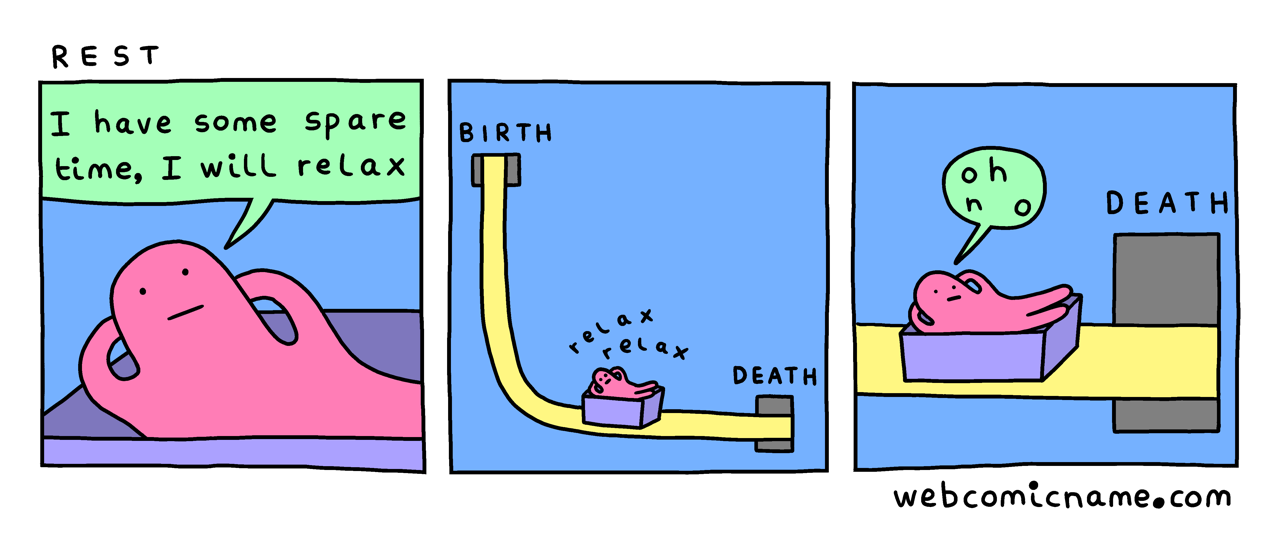
\includegraphics[width=0.85\textwidth]{procrastination.png}
%\end{figure}

\end{document}
